\section{Results}
\label{sec:results}

Table~\ref{tab:accuracy} summarises the accuracy of each method on the 256 test instances, and Table~\ref{tab:cost} its cost.

\begin{table}[t]
\centering
\caption{Accuracy on 256 test instances: median over instances, with the maximum in parentheses. Errors are against the closed form over the periods up to about 2300.}
\label{tab:accuracy}
\begin{adjustbox}{max width=\textwidth}
\begin{tabular}{lcccc}
\toprule
 & SDDP & Neural SDDP, & Neural SDDP, & Pseudo-state \\
 & & no iterations & warm-started & DEQN \\
\midrule
\multicolumn{5}{l}{\textit{DICE 2016}} \\
SCC, mean relative error (\%) & 0.0007 (0.002) & 0.24 (2.1) & 0.0007 (0.002) & 1.8 (19) \\
SCC in the first period, relative error (\%) & 0.00001 (0.0008) & 0.37 (3.3) & 0.00001 (0.0008) & 2.0 (21) \\
Mean $|\mu - \mu^*|$ & 0.00001 (0.00003) & 0.0003 (0.003) & 0.00001 (0.00003) & 0.003 (0.028) \\
Max $|x - x^*|$ & 0.00002 (0.00005) & 0.00003 (0.00007) & 0.00002 (0.00005) & 0.006 (0.051) \\
Welfare loss (\%) & $<10^{-7}$ & $<0.0002$ & $<10^{-7}$ & -- \\
\midrule
\multicolumn{5}{l}{\textit{DICE 2023}} \\
SCC, mean relative error (\%) & 0.0007 (0.002) & 0.21 (2.5) & 0.0007 (0.002) & 4.0 (35) \\
SCC in the first period, relative error (\%) & 0.00001 (0.0008) & 0.26 (4.2) & 0.00001 (0.0008) & 3.6 (33) \\
Mean $|\mu - \mu^*|$ & 0.00001 (0.00002) & 0.0003 (0.004) & 0.00001 (0.00002) & 0.011 (0.059) \\
Max $|x - x^*|$ & 0.00002 (0.00003) & 0.00003 (0.0001) & 0.00002 (0.00004) & 0.010 (0.047) \\
Welfare loss (\%) & $<10^{-7}$ & $<0.0006$ & $<10^{-7}$ & -- \\
\bottomrule
\end{tabular}
\end{adjustbox}
\end{table}

\begin{table}[t]
\centering
\caption{Cost per test instance (median, one process) and training cost. Times for the two calibrations differ by less than 10\%; the table shows DICE 2016.}
\label{tab:cost}
\begin{tabular}{lccc}
\toprule
 & Iterations & Stage problems & Seconds \\
\midrule
SDDP from scratch & 2 & 1{,}350 & 2.5 \\
Neural SDDP, no iterations & -- & 450 & 0.9 \\
Neural SDDP, warm-started & 2 & 1{,}350 & 2.6 \\
\midrule
\multicolumn{4}{l}{\textit{Training (wall time on four cores)}} \\
SDDP solutions of 128 training instances & & & 90 \\
Cut network & & & 672 \\
Pseudo-state DEQN, for comparison & & & 3{,}170 \\
\bottomrule
\end{tabular}
\end{table}

\subsection{SDDP reproduces the closed form}

SDDP converges after two iterations on every instance, as Corollary~\ref{cor:two} predicts, with 1{,}350 stage problems: two forward passes and one backward pass over 450 stages. Its SCC matches the closed form to within 0.002\% on every test instance, its abatement rate to within $3 \times 10^{-4}$ and its consumption rate to within $5 \times 10^{-5}$ in every period; these residual errors are the solver's tolerance. The cut slopes agree with \eqref{eq:bk}--\eqref{eq:bM}: over the evaluation window, the largest relative deviation of any slope is $10^{-15}$ at baseline parameters and $8 \times 10^{-4}$ at the lowest discount rate and highest damages, where the truncation of Remark~\ref{rem:truncation} remains. The baseline SCC in 2050 is \$36.98 per tCO$_2$ for DICE 2016 and \$41.99 for DICE 2023, equal to the closed form to the cent.

Table~\ref{tab:truncation} shows why the horizon has to be long. With the lowest discount rate and the highest damages, a horizon of 150 periods leaves a mean SCC error of 4.2\% over the evaluation window, and 100 periods an error of 15\%; 450 periods bring it to 0.002\%. At the baseline and at high discount rates, 150 periods already suffice. The errors decay roughly like $\beta^{T-58}$, as Remark~\ref{rem:truncation} predicts.

\begin{table}[t]
\centering
\caption{Mean relative SCC error over the evaluation window (\%) for different horizons, DICE 2016.}
\label{tab:truncation}
\begin{tabular}{lccccc}
\toprule
Horizon $T$ (periods) & 100 & 150 & 250 & 350 & 450 \\
\midrule
$\rho = 0.5\%$, $\xi_0 \times 2$, $\omega = 0.75$ & 15.0 & 4.2 & 0.32 & 0.024 & 0.002 \\
Baseline & 0.027 & 0.0006 & 0.0005 & 0.0006 & 0.0006 \\
$\rho = 3.5\%$, $\xi_0 \times 0.5$, $\omega = 1.25$ & 0.007 & 0.0007 & 0.0004 & 0.0006 & 0.0006 \\
\bottomrule
\end{tabular}
\end{table}

\subsection{Neural SDDP without iterations}

A single forward pass with the predicted cuts gives the SCC with a median error of 0.24\% for DICE 2016 and 0.21\% for DICE 2023, and at most 2.1\% and 2.5\%; the abatement rate is within 0.0003 of the optimum in the median, and the welfare loss is below 0.0006\% on every test instance (Table~\ref{tab:accuracy}). The predicted SCC in the first period tracks the closed form across its full range, from about \$5 to \$140 per tCO$_2$ (Figure~\ref{fig:parity}), and the predicted paths of abatement and the SCC follow the closed form to 2200, including the period in which abatement reaches 100\% (Figure~\ref{fig:paths}). As for the deep equilibrium net, the largest errors occur at low time preference: the median SCC error is 0.5\% for $\rho \le 1\%$ and 0.2\% elsewhere (Figure~\ref{fig:accuracy}). A forward pass costs a third of an SDDP solution: 450 stage problems instead of 1{,}350, and 0.9 seconds instead of 2.5. Predicting the cuts takes 7 milliseconds.

\begin{figure}[t]
\centering
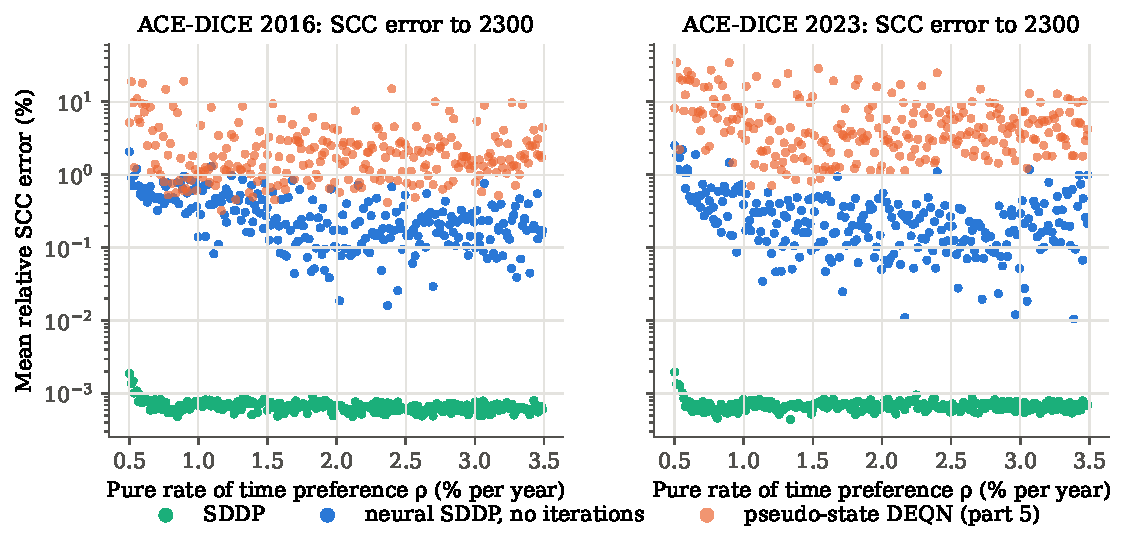
\includegraphics[width=\textwidth]{accuracy.pdf}
\caption{Mean relative SCC error over the evaluation window on the 256 test instances, against the time preference, for SDDP, neural SDDP without iterations, and the pseudo-state deep equilibrium net. Log scale.}
\label{fig:accuracy}
\end{figure}

\begin{figure}[t]
\centering
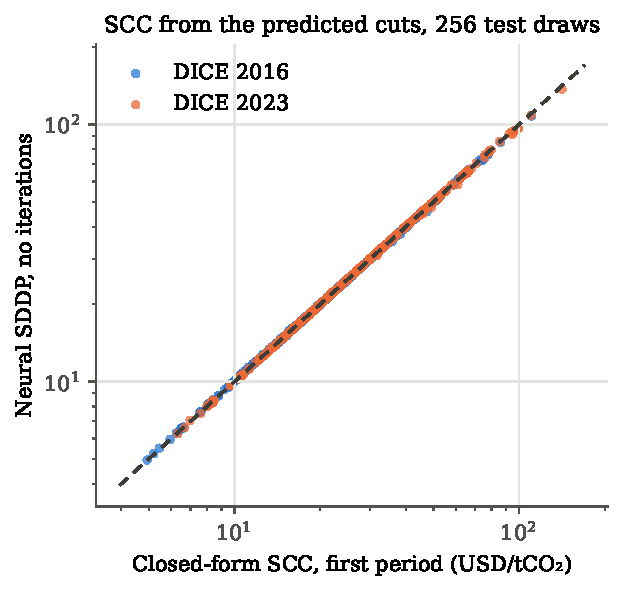
\includegraphics[width=0.55\textwidth]{parity.pdf}
\caption{SCC in the first period from the predicted cuts, against the closed form, on the 256 test instances of both calibrations.}
\label{fig:parity}
\end{figure}

\begin{figure}[t]
\centering
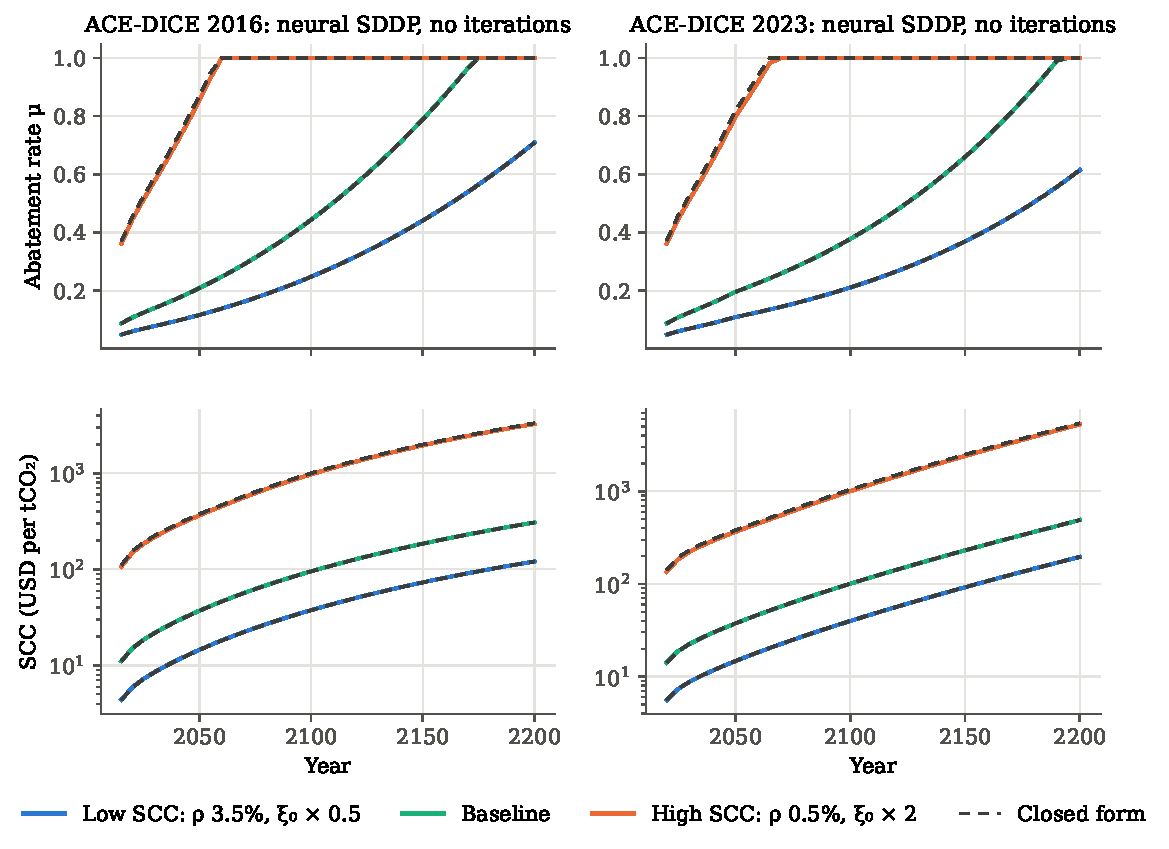
\includegraphics[width=\textwidth]{paths.pdf}
\caption{Abatement rate and SCC from neural SDDP without iterations (solid) and the closed form (dashed), for three instances: low SCC ($\rho = 3.5\%$, half the baseline damages), baseline, and high SCC ($\rho = 0.5\%$, twice the baseline damages).}
\label{fig:paths}
\end{figure}

\subsection{Comparison with a pseudo-state deep equilibrium net}

On the same test instances, the pseudo-state deep equilibrium net has a median SCC error of 1.8\% for DICE 2016 and 4.0\% for DICE 2023, and at most 19\% and 35\%. Neural SDDP without iterations is 8 to 19 times more accurate in the median and 9 to 14 times in the worst case, and its abatement errors are 10 to 35 times smaller (Table~\ref{tab:accuracy}, Figure~\ref{fig:accuracy}). Its training is also cheaper: 90 seconds of SDDP for the training data and 11 minutes for the network, against 53 minutes for the deep equilibrium net (38 minutes for DICE 2023), all on four CPU cores. Section~\ref{sec:discussion} discusses why this comparison favours neural SDDP.

\subsection{Warm starts}

\begin{figure}[t]
\centering
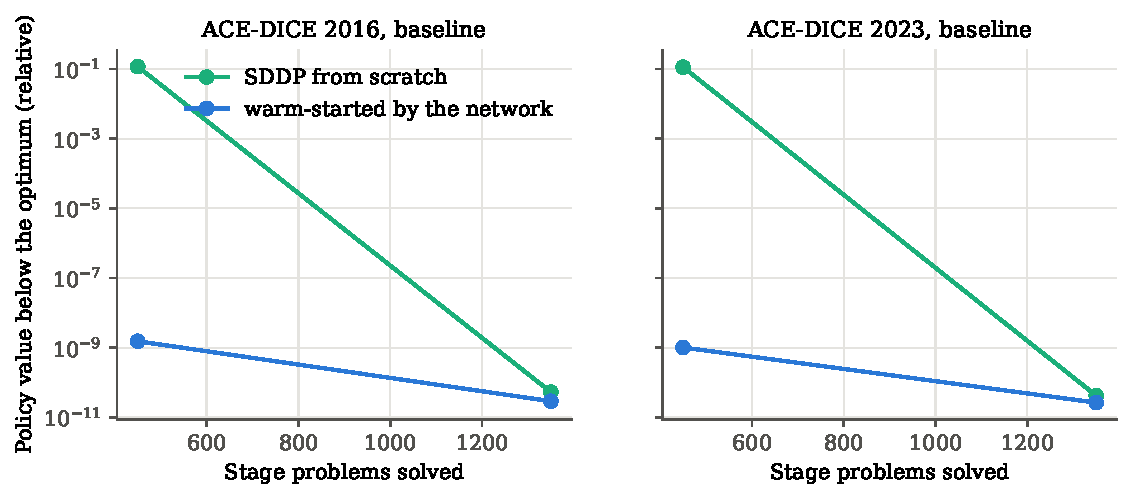
\includegraphics[width=\textwidth]{convergence.pdf}
\caption{Relative shortfall of the forward-pass value from the optimum at baseline parameters, against the number of stage problems solved, for SDDP from scratch and warm-started with the predicted cuts. Log scale; each marker is one iteration.}
\label{fig:convergence}
\end{figure}

With the predicted cuts, the first forward pass is already nearly optimal: its value is within $1.5 \times 10^{-9}$ (DICE 2016) and $1.0 \times 10^{-9}$ (DICE 2023) of the optimum, against 11.7\% below it for SDDP from scratch, whose first forward pass is driven only by the provisional bound (Figure~\ref{fig:convergence}). But the predicted cuts are not guaranteed to lie above the value function, so they cannot certify convergence; a backward pass is needed either way. SDDP from scratch needs exactly one (Corollary~\ref{cor:two}), and both variants finish after two iterations, with the same 1{,}350 stage problems and the same accuracy (Table~\ref{tab:cost}).

\subsection{Productivity shocks}

With i.i.d.\ shocks to log productivity with a standard deviation of 3\%, SDDP runs six iterations of 2{,}700 stage problems each (16{,}200 in total, 31 seconds): forward passes along sampled shocks and backward passes over five Gauss--Hermite nodes. The cut slopes match the closed form to $10^{-14}$, and along a sampled path, on which log capital deviates from the deterministic optimum by up to 0.07, the decisions match the deterministic optimal policy to within $3 \times 10^{-5}$ for the consumption rate and $10^{-4}$ for the abatement rate. As ACE predicts, the shocks shift the value function but not its slopes, and with it, not the policy.
